%%%%%%%%%%%%%%%%%%%%%%%%%%%%%%%%%%%%%%%%%%%%%%%%%%%%%%%%%%%%%%%%%%%%%%%%%%%%%%%%%%
\begin{frame}[fragile]\frametitle{}
\begin{center}
{\Large Instructions}
\end{center}
\end{frame}


%%%%%%%%%%%%%%%%%%%%%%%%%%%%%%%%%%%%%%%%%%%%%%%%%%%%%%%%%%%%%%%%%%%%%%%%%%%%%%%%%%
\begin{frame}[fragile]\frametitle{Preparation}
    \begin{itemize}
        \item Lie in Shavasana (शवासन).
        \item Bring your awareness to the space between your body and the earth.
        \item Let your body soften and sink into the floor.    
	\end{itemize}
	
      \begin{center}
        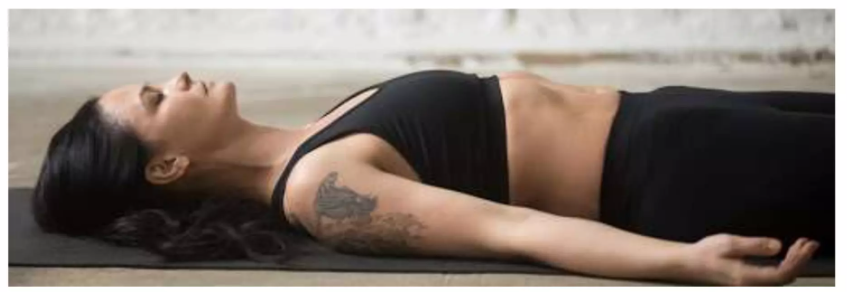
\includegraphics[width=\linewidth,keepaspectratio]{yoganidra7}

		{\tiny (Ref: Yoga Nidra - Dr Amit Chail)}		
        \end{center}	
\end{frame}

%%%%%%%%%%%%%%%%%%%%%%%%%%%%%%%%%%%%%%%%%%%%%%%%%%%%%%%%%%%%%%%%%%%%%%%%%%%%%%%%%%
\begin{frame}[fragile]\frametitle{Setting the Sankalpa (संकल्प)}
    \begin{itemize}
        \item A positive “I am” statement to guide your Yoganidra practice.
        \item Examples:
        \begin{itemize}
            \item "I am strong."
            \item "I am peaceful."
            \item "I am the witness."
        \end{itemize}
        \item Repeat the Sankalpa 3 times at the start and end of Yoganidra.
    \end{itemize}
\end{frame}

%%%%%%%%%%%%%%%%%%%%%%%%%%%%%%%%%%%%%%%%%%%%%%%%%%%%%%%%%%%%%%%%%%%%%%%%%%%%%%%%%%
\begin{frame}[fragile]\frametitle{Rotation of Awareness (Abbreviated)}
    \textbf{Focus on body parts:}

\begin{columns}
    \begin{column}[T]{0.6\linewidth}
    \begin{itemize}
        \item Right heel
        \item Left heel
        \item Right calf
        \item Left calf
        \item Right knee
        \item Left knee
        \item Right thigh
        \item Left thigh
        \item Both hips
        \item Lower back
        \item Upper back
        \item Right shoulder
        \item Left shoulder
        \item Back of the head
    \end{itemize}

    \end{column}
    \begin{column}[T]{0.4\linewidth}
	      \begin{center}
        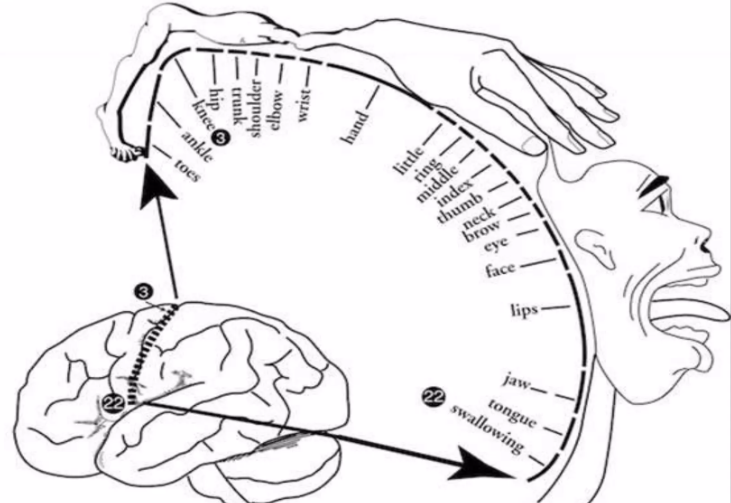
\includegraphics[width=\linewidth,keepaspectratio]{yoganidra8}

		{\tiny (Ref: Yoga Nidra - Dr Amit Chail)}		
        \end{center}
    \end{column}
  \end{columns}
  
  

	
	
\end{frame}

%%%%%%%%%%%%%%%%%%%%%%%%%%%%%%%%%%%%%%%%%%%%%%%%%%%%%%%%%%%%%%%%%%%%%%%%%%%%%%%%%%
\begin{frame}[fragile]\frametitle{Breath Awareness}
    \textbf{Breath Visualization:}
    \begin{itemize}
        \item Visualize breath as golden light flowing up and down the spine.
        \item Inhale: light rises from the tailbone to the crown.
        \item Exhale: light flows back down.
        \item Feel the cosmic flow of prana (प्राण).
    \end{itemize}
\end{frame}

%%%%%%%%%%%%%%%%%%%%%%%%%%%%%%%%%%%%%%%%%%%%%%%%%%%%%%%%%%%%%%%%%%%%%%%%%%%%%%%%%%
\begin{frame}[fragile]\frametitle{Opposite Sensations}
    \begin{itemize}
        \item Bring awareness to the sensation of heat
        \item Feel your whole body becoming warm.
        \item Shift awareness to cold. Feel the entire body cooling down.
        \item Release both sensations.
		\item Similarly: heaviness and lightness, pain and pleasure, love and hate, etc
    \end{itemize}
\end{frame}

%%%%%%%%%%%%%%%%%%%%%%%%%%%%%%%%%%%%%%%%%%%%%%%%%%%%%%%%%%%%%%%%%%%%%%%%%%%%%%%%%%
\begin{frame}[fragile]\frametitle{Guided Imagery}
    \textbf{Journey through Nature:}
    \begin{itemize}
        \item Imagine standing in a meadow, surrounded by a lush forest.
        \item Feel the warmth of the sun and smell the wildflowers.
        \item Walk into the forest, following a path that leads uphill.
        \item Reach a cave and discover a lit candle inside.
        \item Meditate on the candle's flame, with your Sankalpa inscribed on it.
    \end{itemize}
\end{frame}

%%%%%%%%%%%%%%%%%%%%%%%%%%%%%%%%%%%%%%%%%%%%%%%%%%%%%%%%%%%%%%%%%%%%%%%%%%%%%%%%%%
\begin{frame}[fragile]\frametitle{Exiting the Practice}
    \begin{itemize}
        \item Repeat your Sankalpa 3 times.
        \item Bring awareness to the sounds around you.
        \item Slowly move and break Shavasana.
    \end{itemize}
\end{frame}
